
\documentclass[journal,twoside]{IEEEtran}
\usepackage{cite}
\usepackage[pdftex]{graphicx}
\graphicspath{{./classe/}}
\DeclareGraphicsExtensions{.pdf,.jpeg,.png,.jpg}
\usepackage{amsmath}
\usepackage{algorithmic}
\usepackage{array}
\usepackage{url}
    \begin{document}
    \setcounter{page}{33}
    \title{Design and Performance Analysis of Highly Efficient\\Class E Resonant Inverter*\thanks{*Class E Resonant Inverter and Class E RF Amplifier are used interchangeably in this paper. The only difference
in naming depends on its field of application.}}
    \author{{~Ashutosh~Timilsina,~    Beni~Nepali,~Binay~Paudyal,~and~Jenesha~D.~Kunwar}\\
    \IEEEauthorblockA{Department of Electrical Engineering, Institute of Engineering, Tribhuvan University, Pulchowk, Lalitpur, Nepal }}


\markboth{Zerone Scholar,~Vol.~1, No.~1, November~2016}%
{Timilsina \MakeLowercase{\textit{et al.}}: Design and Performance Analysis of Class E Resonant Inverter}

    \maketitle
	\begin{abstract}
This paper focuses on designing of a highly efficient Class E Power Inverter which does not take into account transistor
parasitic effects. It is assumed that the transistor parasitic effects do not produce any large difference in output. This
inverter operates on nearly zero power loss at switching instant whereas at normal operation, there always exists a phase
shift between voltage and current, whose product will be negligibly small. Hence, the result is a highly efficient power
inverter which is useful in high frequency operation.
	\end{abstract}
	\begin{IEEEkeywords}
Class E Resonant Inverter, GaN HEMT, High Frequency Amplifier
	\end{IEEEkeywords}
	\section{Introduction}
\IEEEPARstart{H}{}igh frequency operation has been gaining strong attention
and popularity among researchers currently. Different
electrical and electronic equipment are being upgraded that
includes its operation in HF region. Wireless communication
has already been established and the wireless power transfer
technology is gaining wide acceptance which also uses high
frequency signal for efficient power transmission utilizing
strongly coupled magnetic resonance \cite{Kurs2007}. High switching
losses occur in devices operating at high frequency as
compared to the devices operating at low frequency because
of quick change in polarity, high frequency noise, harmonics,
and transients during high frequency operation. In case of
wireless power transfer, the power loss has to be eliminated
wherever possible as it increases the efficiency of the overall
system \cite{Fu2013}. The Class E RF Amplifier, introduced
by Sokal et al in 1972, is generally used for the purpose of
Wireless Power Transfer and for numerous RF applications
\cite{Klehn2009}.
\section{Operating Principle and Theory}
Unlike class A, AB and push pull inverters, a Class E inverter
is supposed to have 100\% efficiency (theoretically). Another
benefit of using Class E inverter is that it uses only one power
switching device that reduces cost and overall loss since
major loss occurs on the switching devices and cost of the
switching devices is larger than other components used in a
power inverter.\\

Even though transistor parasitic effect is not considered in this
design, its effect increases on increasing the operating
frequency. According to \cite{Sokal2001}, the shunt capacitance, along with
the capacitance between drain and source of the switching
devices ($C_{ds}$ ), limits the operating frequency and a high value
of C ds prevents the amplifier from achieving Zero Voltage
Switching (ZVS). Hence 100\% efficiency is not achieved. For
high frequency, only $C_{ds}$ (parasitic capacitance) is sufficient
for operation. Class E amplifier maintains the wave shape of
the current and voltage across the switching devices so high
amount of power will not be dissipated that reduces the loss in
switching devices.\\
For switching operation, MOSFET and transistor both can be
used but they should have high switching capacity of 10-
20MHz or more. Switching frequency also affects the value
of shunt capacitor used since before the device is switched, it
is necessary for the shunt capacitor to discharge completely.\\

\begin{figure}[!ht]
\centering
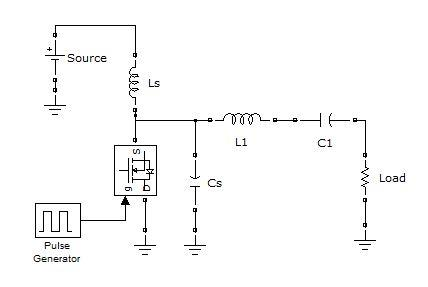
\includegraphics[width=2.5in]{1}
\caption{Schematic diagram of Class E Inverter}
\label{fig_1}
\end{figure}


Fig~\ref{fig_1} shows the schematic diagram of the Class E inverter. A
function generator is used to drive the MOSFET which is
used as switching device to generate pulse of specific
frequency. The duty cycle of pulse is 0.5. A constant DC
supply is provided to the source of switching device through
the choke inductor ($L_s$ ). $L_s$ is used to regulate the current in
amplifier. The series resonant circuit $L_1$ and $C_1$ are made to
resonate at switching frequency which offers low impedance
in circuit and prevents high frequency harmonics.\\
In a Class E inverter, three types of capacitances are involved
within the MOSFET itself:
input capacitance, output
capacitance and transfer capacitance \cite{ClassRadio}. Input capacitance is
the capacitance appearing at the gate terminal of the
MOSFET and it prevents the switching device (MOSFET) to
drive easily in high frequency. This value is very high for
MOSFET so it almost acts as short circuit in vacuum. Its
effect can be removed by making it a part of the resonant
circuit or by using autotransformer. The output capacitance
plays major role in the Class E inverter because this
capacitance is responsible to get efficient sinusoidal output.
The self-capacitance (parasitic capacitance) of the MOSFET
appearing at the drain-source terminal is the output
capacitance. In fig~\ref{fig_1}, $C_s$ is the output capacitor which is in
shunt with the parasitic capacitance. This capacitor has to be
discharged completely before the device is switched to “ON”
state. Therefore, the discharging time has to match with the
switching time of the device. The other capacitance is the
transfer capacitance which the capacitance between the drain
and the gate. It stops the MOSFET from operating in high
frequency when high voltage is at drain. Nowadays,
manufacturing companies design MOSFETs which have a
reduced transfer capacitance which means that this does not
create any trouble during operation.\\

Class E inverter operates in either “ON” or “OFF” state
according to the state of the switching device. A pulse of
required frequency is supplied to the gate terminal. The high
level of pulse activates the switching device which is known
as “ON” state whereas the low level of pulse deactivates the
switching device which is known as “OFF” state.
\lq\lq OFF\rq\rq state
At this state, the switching device acts as an open circuit
which means that no current flows through the switching
device. Hence, all of the current flows through the capacitor
($C_s$ ) and load (through series resonant circuit). Then the
capacitor starts to charge. The voltage supplied at capacitor is higher than normal supply voltage so the output obtained is in
amplified form.\\
\begin{figure}[!ht]
\centering
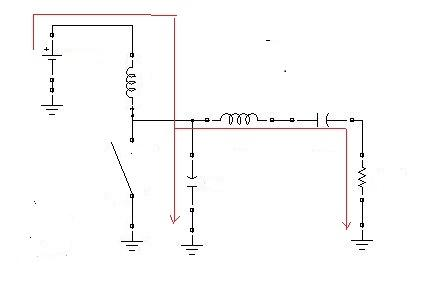
\includegraphics[width=2.5in]{2}
\caption{OFF state of the switching devices}
\label{fig_2}
\end{figure}

The red line in fig~\ref{fig_2} denotes the flow of current during OFF
state.
\lq\lq ON\rq\rq state
At this state, the switching device acts as a short circuit so the
DC supply flows through the low impedance path i.e. through
the device. At that time the choke inductor, $L_s$ starts charging
which will be discharged at “OFF” state as mentioned earlier.
At this instant, the capacitor is fully charged so it will supply
the potential to the low impedance path. Now, the capacitor
voltage with the DC supply voltage will return from the
opposite direction of the previous supply in the load. Due to
this reason, positive and negative polarity is established at the
load.


\begin{figure}[!ht]
\centering
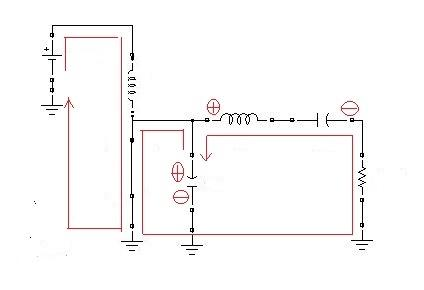
\includegraphics[width=2.5in]{3}
\caption{ON state of switcing devices}
\label{fig_3}
\end{figure}
The red line denotes the current flow in fig~\ref{fig_3}.



\section{Design and Result}

Finding out the value of different component analytically is a
complex task but there is an empirical formula available with
which the value of the different components can be easily
calculated. The following are the formulae to find out the
parameters as derived in \cite{Sokal2001}.

\begin{align}
R_L= \frac{(V_{cc}-V_0)^
2}{P}*0.576801*(1.001245-\notag
\\ \qquad \frac{0.451759}{Q_L}-\frac{0.402444}{Q_L^2})
\end{align}

\bigskip

Where $R_L$ = Load, $V_0$ = saturation voltage whose value is 0
for FET, P = power to be delivered and $Q_L$ = Quality factor.
The shunt capacitance across the drain-source terminal is
given by following equation.

\begin{align}
C_s= \frac{1}{2\pi fR_L(\frac{\pi ^2}{4}+1)\frac{\pi}{2}}(0.9986+ \frac{0.91424}{Q_L}-\notag\\ \qquad\frac{1.03175}{Q_L^2}) +\frac{0.6}{(2\pi f)^2L_c}
\end{align}

\bigskip

Where $L_s$ = choke inductor. Equation (2) is used to find out
the shunt capacitor. Output capacitance is taken as a
combination of shunt capacitance and parasitic capacitance.
The capacitance of the series resonant circuit which also
function as filter circuit is given by
\begin{align}
C_1=\frac{1}{2\pi fR_L}(\frac{1}{Q_L-0.104823})(1.00121+\notag\\\qquad\qquad\frac{1.01468}{Q_L-1.7879})-\frac{0.2}{(2\pi f)^2L_s}
\end{align}


\bigskip
Equation (3) is used to find out the value of the capacitor
which is the part of series resonant circuit. The inductance of
the series resonant circuit is determined by following equation

\begin{equation}
L_1=\frac{Q_LR}{2\pi f}
\end{equation}

\bigskip
Equation (4) is used to find the inductance value which is in
series with the capacitor of resonant circuit. The inductor and
capacitor prevent high frequency harmonics in the circuit.
The value of $V_cc$ , P and $Q_L$ can be specified beforehand.
Other empirical formulae to calculate the parameters are as
follows:

\begin{equation}
L_s=\frac{0.4001R}{\omega _s}
\end{equation}


\bigskip
where R is the load resistance. $L_s$ is the inductance of choke
inductor and $\omega _s$ is the frequency of supply.

\begin{equation}
C_s=\frac{2.165}{R\omega _s}
\end{equation}

\bigskip
Where, $C_s$ is the simpler form of shunt capacitance as
represented by equation (2) as presented in [6]. Also another
empirical formula presented in [6] is

\begin{equation}
\omega _sL_1-\frac{1}{\omega _sC_1}=0.3553R
\end{equation}


\bigskip

Where, $L_1$ and $C_1$ are the capacitance and inductances of
capacitor and inductor respectively of the resonant circuit.
Using above empirical formulae, a simulation is done in
MATLAB which is shown in fig1 in which the value of
parameter are taken as $R_L$ = 20 ohm, choke inductor ($L_s$) =
130 $\mu$H , shunt capacitance ($C_s$) = 1.27 nF , resonant
capacitor ($C_1$) = 10.5 pF and resonant inductor ($L_1$) = 10 $\mu$ H .
The pulse generator generates frequency of 10 MHz which is
injected to the gate terminal of MOSFET and the waveform
of voltage and current in the load is obtained as shown in fig~\ref{fig_4}.
\begin{figure}[!ht]
\centering
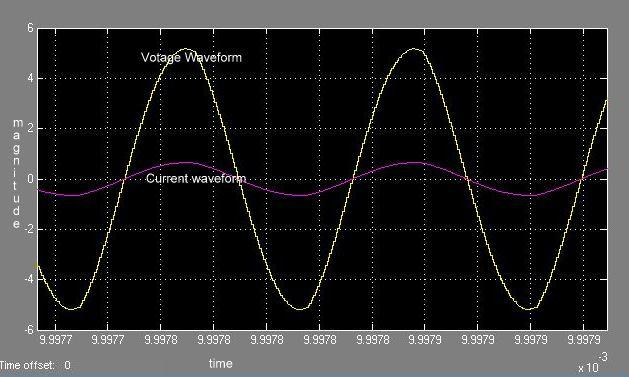
\includegraphics[width=2.5in]{4}
\caption{Simulation result of class E amplifier}
\label{fig_4}
\end{figure}
Fig~\ref{fig_4} represents the output obtained by Class E amplifier in
MATLAB simulation. The larger waveform represents
voltage waveform and smaller waveform represents current
waveform. The input to the circuit is 5V dc and output voltage is ac voltage of 13.56MHz as the gate signal for
driving the MOSFET was fed at same frequency.
Same Class E Power Inverter circuit was realized in the
hardware to examine and compare the performance of the
simulated and actual circuit. It is difficult to realize the
components of the exact rating as presented in the simulation,
however, approximate value of component is used and the
designed Class E amplifier circuit is shown in fig~\ref{fig_5}.
\begin{figure}[!ht]
\centering
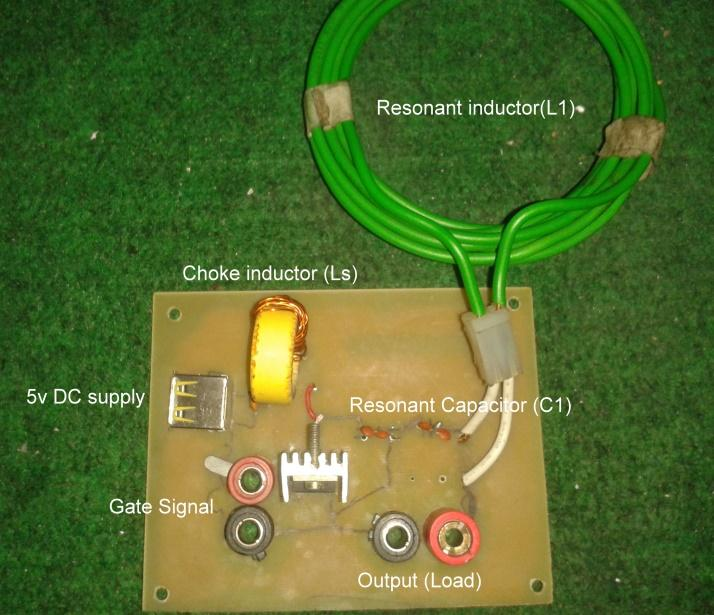
\includegraphics[width=2.5in]{5}
\caption{Class E Power Inverter}
\label{fig_5}
\end{figure}

As a switching device, IRFZ44N MOSFET from International
Rectifier is used which has a fast switching capability upto 70
KHz frequency. Another MOSFET from International
Rectifier IRF1010E has switching capability of upto 60MHz
frequency which can also be used for this circuit. In recent
days GaN HEMT is also gaining popularity among high
frequency applications. 5V DC was supplied to the Class E
inverter through USB port. Choke inductor of value 100 $\mu$ H
and a shunt capacitor of capacitance 1nF have been used. The
resonant circuit which consists of a capacitor and inductor of
10 pF and 12.9 $\mu$ H respectively has been used. The gate
signal is provided from a function generator that can provide
up to 14 MHz. The output waveforms of voltage and current
are observed in oscilloscope.




\begin{figure}[!ht]
\centering

\includegraphics[width=2.5in]{6}
\caption{Waveform of output of Class E Amplifier}
\label{fig_6}
\end{figure}

Fig~\ref{fig_6} shows the output from the Class E inverter in an
oscilloscope. Due to use of a higher inductance coil, there
exists a phase difference between the current and voltage. The
simulation waveform and real waveform seemed to have
matched in shape. The output obtained has a frequency equal
to the switching frequency which is 70 KHz. If $C_s$ is within
about 10\% of the intended value, it won't need any
adjustment. The adjustment procedure for optimum
performance of the circuit followed was as described in \cite{Sokal2001}.
The output waveform of hardware and simulation were
similar in nature but different in magnitude. The practical
circuits have limitation due to inductive coupling between
inductors, parasitic capacitance, delay in switching of the
MOSFET which have differed the output from desired value.
Also the parasitic effects of the interconnects cannot be
neglected in real circuit.



\section{Conclusion}
Class E Resonant Inverter produces highly sinusoidal
waveforms as output with very less distortions. Since the
transistor is used as switching device, the power loss incurred
in the circuit is largely reduced. With increase in frequency
the operation of amplifier and inverter circuit is affected and
to overcome this problem Class E RF Amplifier (or Class E
Resonant Inverter) can be used which can be used up to 10
GHz depending on the type of transistor used. Also it was
observed that the efficiency of the class e resonant inverter is
higher compared to other amplifier. The presented resonant
inverter can be applied for several configurations by changing
the circuit parameters and following the adjustment procedure
as in \cite{Sokal2001}.


\begin{thebibliography}{9}

\bibitem{Kurs2007} 
    A. Kurs, A. Karalis, R. Moffatt, J.D. Joannopoulos, P. Fisher and M. Soljacic, \textit{Wireless Power Transfer
    via Strongly Coupled Magnetic Resonances}, Science 317, 83, 2007.
\bibitem{Fu2013}
    M. Fu, T. Zhang, X. Zhu and C. Ma, \textit{A 13.56 MHz wireless power transfer system without impedance
    matching networks}, Wireless Power Transfer (WPT), 2013 IEEE, Perugia, 2013, pp. 222-225.
\bibitem{Klehn2009}
    B. Klehn, \textit{A Precise Analysis of a Class E Amplifier},Thesis, Rochester Institute of Technology, 2009.
\bibitem{Sokal2001}
    N.O. Sokal, \textit{Class-E RF Power Amplifiers}, QEX, January/ February 2001, pp. 9-20.
\bibitem{ClassRadio} 
    “Class E RF Amplifier Theory of Operation,” Class E Transmitters. 
    [Online]. Available: http://www.classeradio.com/theory.htm. [Accessed: 05-June-2016].
\bibitem{Rashid2013}
    M. H. Rashid, \textit{Power Electronics: Circuits, Devices \& Applications}, Pearson Publishers, $4^{th}$ edition, 2013.

\end{thebibliography}


\begin{IEEEbiography}[{
\includegraphics[width=1in,height=1.25in,clip,keepaspectratio]{at}}]{Ashutosh Timilsina}
Ashutosh Timilsina (b. 7th December 1995) is currently working towards his Bachelor in Electrical Engineering at Tribhuwan University, Institute of Engineering (IoE), Pulchowk Campus Nepal. An enthusiast in Quantum Mechanics, Electromagnetism, Power System Designing and Wireless Power Transfer Systems; he completed his research experience for undergraduates at IoE in Summer 2016 under the supervision of Dr. Arbind Kumar Mishra entitled "Wireless Power Transfer Based System via Strongly Coupled Magnetic Resonance" for which he co-authored a thesis. During the School year 2012-2016, he was involved in several projects related to electrical engineering including Wireless Power Transfer System, Tesla Coil, Cockcroft-Walton High Voltage Generator, and Automatic Greenhouse System. He was also the winner of Electrical Event Category of LOCUS 2015 for Cockcroft-Walton HV Generator. His research interests lie in Wireless Power, Transmission and Distribution Designing, High Voltage Engineering, Energy Harvesting,Language and Linguistics and Artificial Neural Network. Mr. Timilsina is a member of Electrical Club, a fraternity at IoE and has served as Editor for Zerone Magazine and Scholar under LOCUS 2016.
\end{IEEEbiography}

\newpage
\begin{IEEEbiography}[{
\includegraphics[width=1in,height=1.25in,clip,keepaspectratio]{bn}}]{Beni Nepali}
was born in June 4,
1995. He did his Bachelors in Electrical Engineering
from Pulchowk Campus, IOE, Pulchowk. His fields of interests include Electrical Machines, Power generation and Power transmission and distribution. 
\end{IEEEbiography}


\begin{IEEEbiography}[{
\includegraphics[width=1in,height=1.25in,clip,keepaspectratio]{bp}}]{Binay Paudyal}
was born in July 12,
1995. He did his Bachelors in Electrical Engineering
from Pulchowk Campus, IOE, Pulchowk. His fields of interests include Electronics and Control System.
\end{IEEEbiography}


\begin{IEEEbiography}[{
\includegraphics[width=1in,height=1.25in,clip,keepaspectratio]{jk}}]{Jenesha D. Kunwar}
was born in February 25,
1994. She studied Bachelors in Electrical Engineering
at Pulchowk Campus, IOE, Pulchowk from 2012 to 2016. She is particularly interested in working mechanism of electrical machines and Power \& Control System.
\end{IEEEbiography}





\end{document}

